

\subsection{SPC evaluation}
\label{sec:eval_spc}
The evaluation section is now shifted to examine the images produced by the SPC. The images will be analyzed using a range of methods to examine the performance of the SPC. This section will start with the same evaluations performed in the previous section and will end with two new evaluation, edge response and subsampling ratio. All images captured by the SPC of natural scenes was taken at a distance between 200 to 900 meter on sunny days with some clouds.


\subsubsection{Reconstructed performance Using reference image}
This evaluation is designed to get a measurement of expected image quality with the same metrics used in the synthetic case. As stated before, it is hard to obtain a reference image to the images produced by the SPC. One solution to obtain a reference image is to calculate a homography between images. But there are two problems of just performing a homography to obtain a reference image, the fist on is that, homography estimates the transformation between flat surfaces which excludes most natural images, and the second is that, the estimated homography will not be perfect an thus for example high contrast edges in the images will not match and produce large errors in the performance measurements. To solve these two problems the scene is a flat surface with a printed pattern and to avoid the the error from sharp edges the pattern is constructed with smooth contrast changes. To not complicate this experiment the reference image is the computer generated optimal images which was being transformed to fit the image captured by the SPC.\\[0.1in] 

The reference image which was created using sine functions to avoid edges can be seen in figure~\ref{fig:hom_over_im} and the reconstructed images with different subsampling ratio.   


\begin{figure}[H]
    \centering
\begin{minipage}[h]{0.3\textwidth}
	\vspace*{1cm}
    
\includegraphics[width=1\textwidth]{result/hom/im_ref.png}
    \subcaption{Homography transformed refrence image}
    \label{fig:hom_ref}
\end{minipage}
\begin{minipage}[t]{0.22\textwidth}
    
\includegraphics[width = \textwidth]{result/hom/im_m5.png}
    \subcaption{5\%}
    \label{fig:hom_5}
    
\includegraphics[width = \textwidth]{result/hom/im_m20.png}
    \subcaption{20\%}
    \label{fig:hom_20}
\end{minipage}
\begin{minipage}[t]{0.22\textwidth}
    
\includegraphics[width = \textwidth]{result/hom/im_m10.png}
    \subcaption{10\%}
    \label{fig:hom_10}
    
\includegraphics[width = \textwidth]{result/hom/im_m25.png}
    \subcaption{25\%}
    \label{fig:hom_25}
\end{minipage}
\begin{minipage}[t]{0.22\textwidth}
    
\includegraphics[width = \textwidth]{result/hom/im_m15.png}
    \subcaption{15\%}
    \label{fig:hom_15}
    
\includegraphics[width = \textwidth]{result/hom/im_m30.png}
    \subcaption{30\%}
    \label{fig:hom_30}
\end{minipage}
    \caption{The reconstructed images with subsampling ratios between 5-30\% and the reference image transformed to fit the SPC images using homography.}
    \label{fig:hom_over_im}
\end{figure}

Before the results from the evaluation is presented it is worth noting that the reference image is a perfect simulated reference image, which was not effected by the uneven light source and quality of the print as the reconstructed image from the SPC, which for example can be seen in the edges of the reconstructed images in figure~\ref{fig:hom_5} to \ref{fig:hom_30}. In figure~\ref{fig:hom_score}, PSNR and SSIM has been calculated for each subsampling ratio. 


\begin{figure}[H]
    \centering
\begin{minipage}[t]{0.49\textwidth}
    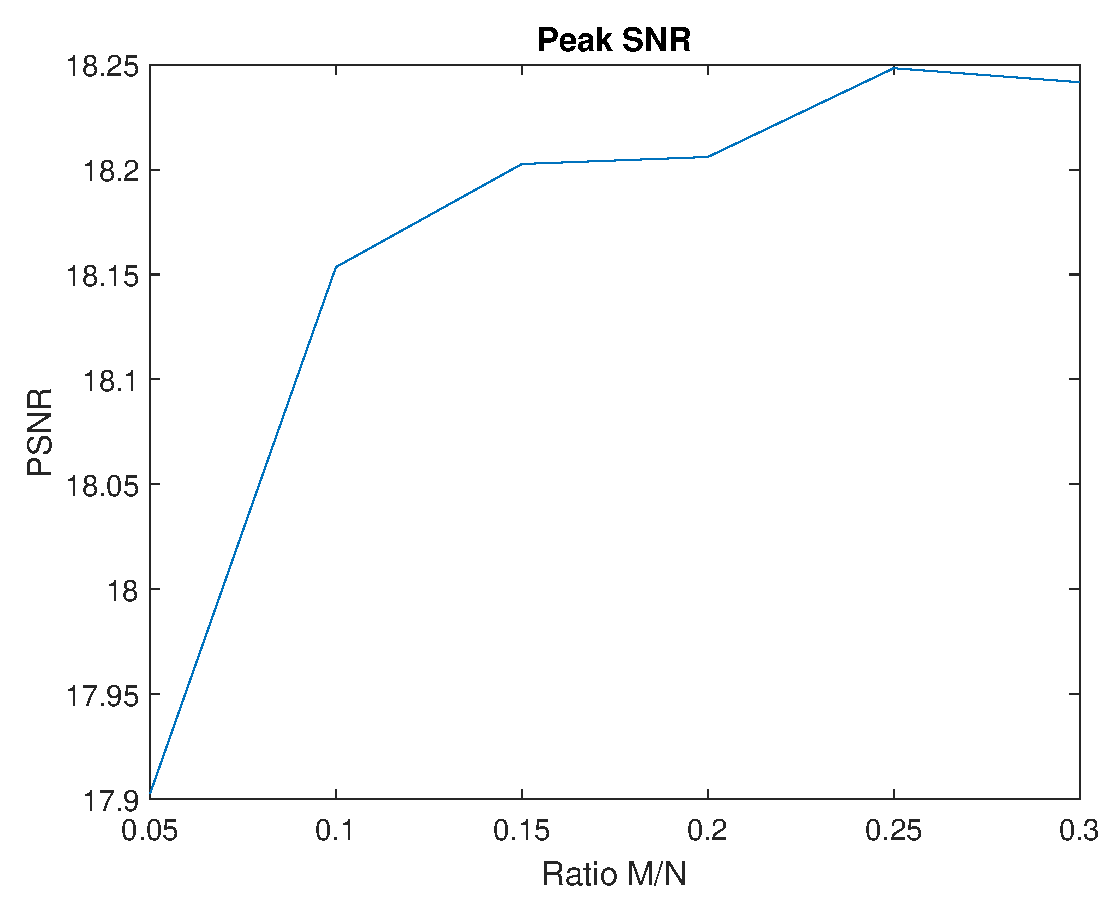
\includegraphics[width=1\textwidth]{result/homo/PSNR_2.eps}
    \subcaption{}
    \label{fig:hom_psnr}
\end{minipage}
\begin{minipage}[t]{0.49\textwidth}
    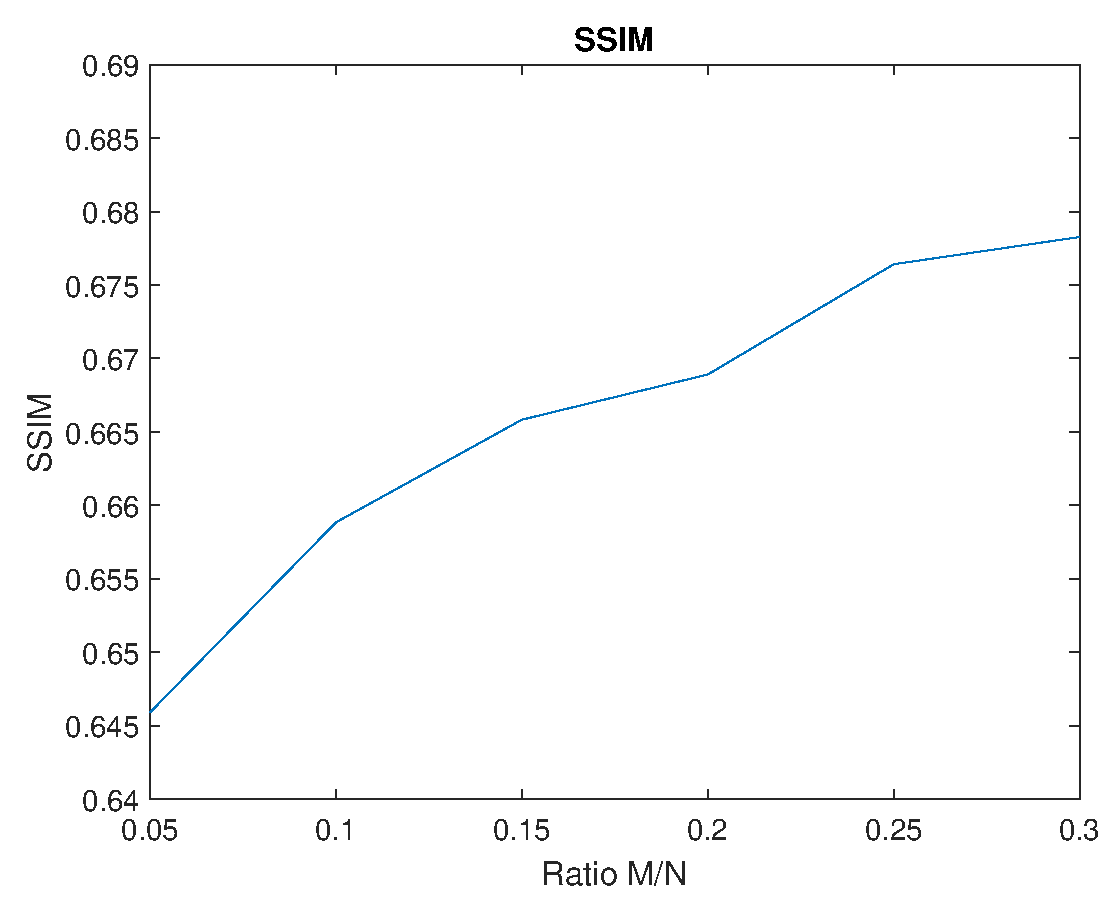
\includegraphics[width=1\textwidth]{result/homo/SSIM_2.eps}
    \subcaption{}
    \label{fig:hom_ssim}
\end{minipage}
    \caption{Signal quality of SPC images compared to reference image. (a) Peak SNR for reconstructed images against reference image. (b) SSIM score for reconstructed images against reference image.}
    \label{fig:hom_score}
\end{figure}

The result shows increased quality with increased subsample ratio. In the case of PSNR the image quality rapidly improves when increasing subsample ratio up to 15\%. 



\subsubsection{Reconstruction performance Using no reference quality assessment}
\label{sec:SPC_BRISQUE}
In this section the blind quality assessment tool BRISQUE is used to evaluate the reconstructed images from the SPC. In addition to presenting the BRISQUE score for the images, each image has been classified into three distinct groups in order to link the BRISQUE scores to each image and their sampled signal.\\[0.1in] 

In figure~\ref{fig:brisque_plot} each image is evaluated using BRISQUE with subsampling rate from $5-30\%$.

\begin{figure}[H]
    \centering
    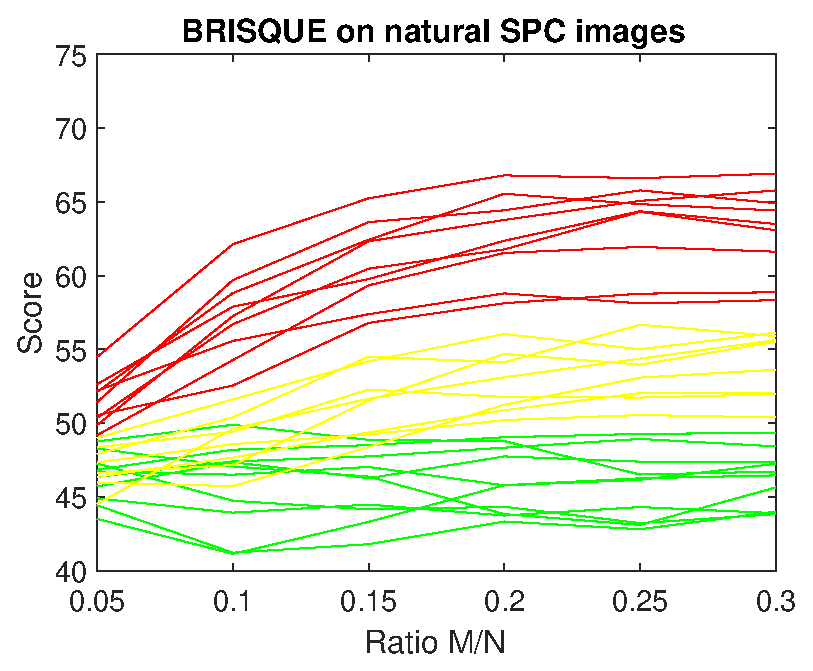
\includegraphics[width = 0.7\linewidth]{result/SPC_NRQA/brisque_spc.eps}
    \caption{BRISQUE score for images reconstructed from the SPC with subsampling ratios from $5\%$ to $30\%$. Each line represent one image and is classified with different colors depending on the initial score at subsampling ratio 5\% and the general trend for higher subsampling ratios. Lower score is better.}
    \label{fig:brisque_plot}
\end{figure}


As seen in figure~\ref{fig:brisque_plot} each image has been plotted separately due the high variance in the image set and the distinct different trends. 


The images has been classified into three different classes depending on the initial score at 5\% subsampling ratio and the trend when increasing the subsampling ratio. The classes has been color coded where:

\begin{itemize}
\item the \textit{red image set} has a higher initial BRISQUE score than the rest of the set and a got worse BRISQUE score at a relative high rate when increasing the subsampling ratio.

\item The \textit{yellow image set} is distinguish by gradual decrease in BRISQUE score when the subsampling ratio is increased.

\item The \textit{green image set} has a plain trend or increased BRISQUE score when the subsampling ratio is increased.
\end{itemize}

 

In figure~\ref{fig:good}-\ref{fig:bad} a subset of four images from each class is presented. All images is reconstructed using 30\% subsampling ratio. 



\begin{figure}[H]
    \centering
\begin{minipage}[t]{0.245\textwidth}
    
\includegraphics[width=1\textwidth]{result/SPC_NRQA/g64_512_m30.PNG}
    \subcaption{}
    \label{fig:good1}
\end{minipage}
\begin{minipage}[t]{0.245\textwidth}
    
\includegraphics[width = \textwidth]{result/SPC_NRQA/g24_512_m30.PNG}
    \subcaption{}
    \label{fig:good2}
\end{minipage}
\begin{minipage}[t]{0.245\textwidth}
    
\includegraphics[width=1\textwidth]{result/SPC_NRQA/g22_512_m30.PNG}
    \subcaption{}
    \label{fig:good3}
\end{minipage}
\begin{minipage}[t]{0.245\textwidth}
    
\includegraphics[width = \textwidth]{result/SPC_NRQA/g65_512_m30.PNG}
    \subcaption{}
    \label{fig:good4}
\end{minipage}
    \caption{Sample images from the green image set.
    (a) and (d) People sitting in the edge of a forest.  (b) Stationary car. (c) Camouflage jackets and a AT-4 anti-tank weapon on the ground.}
    \label{fig:good}
\end{figure}

\begin{figure}[H]
    \centering
\begin{minipage}[t]{0.245\textwidth}
    
\includegraphics[width=1\textwidth]{result/SPC_NRQA/h62_512_m30.PNG}
    \subcaption{}
    \label{fig:half1}
\end{minipage}
\begin{minipage}[t]{0.245\textwidth}
    
\includegraphics[width = \textwidth]{result/SPC_NRQA/h37_512_m30.PNG}
    \subcaption{}
    \label{fig:half2}
\end{minipage}
\begin{minipage}[t]{0.245\textwidth}
    
\includegraphics[width=1\textwidth]{result/SPC_NRQA/h43_512_m30.PNG}
    \subcaption{}
    \label{fig:half3}
\end{minipage}
\begin{minipage}[t]{0.245\textwidth}
    
\includegraphics[width = \textwidth]{result/SPC_NRQA/h35_512_m30.PNG}
    \subcaption{}
    \label{fig:half4}
\end{minipage}
    \caption{Sample images from the yellow image set.
    (a)  People sitting next to a parking lot. (b) - (d) House facades.}
    \label{fig:half}
\end{figure}

\begin{figure}[H]
    \centering
\begin{minipage}[t]{0.245\textwidth}
    
\includegraphics[width=1\textwidth]{result/SPC_NRQA/b20_512_m30.PNG}
    \subcaption{}
    \label{fig:bad1}
\end{minipage}
\begin{minipage}[t]{0.245\textwidth}
    
\includegraphics[width = \textwidth]{result/SPC_NRQA/b46_512_m30.PNG}
    \subcaption{}
    \label{fig:bad2}
\end{minipage}
\begin{minipage}[t]{0.245\textwidth}
    
\includegraphics[width=1\textwidth]{result/SPC_NRQA/b75_512_m30.PNG}
    \subcaption{}
    \label{fig:bad3}
\end{minipage}
\begin{minipage}[t]{0.245\textwidth}
    
\includegraphics[width = \textwidth]{result/SPC_NRQA/b79_512_m30.PNG}
    \subcaption{}
    \label{fig:bad4}
\end{minipage}
    \caption{Sample images from the red image set.
    (a) House facade. (b) Construction crane (Moving clouds in background). (c) Mjärdevi Center facade (Moving clouds reflected in the windows). (d) Mjärdevi Center balcony with people having a break (Moving clouds reflected in the windows).}
    \label{fig:bad}
\end{figure}


As seen in the images in figure~\ref{fig:good} - \ref{fig:bad}, the motive in each class is quite different, the images from the green image set contains forest, people and things, images from the yellow image set contains buildings and structures with horizontal and vertical lines and images from the red image set includes the sky but are also a bit darker and overall noisier. 


The last result in this section is the mean signal strength plotted against the normalized signal variance of the background noise where each signal has the same corresponding color classification as given before.\\[0.1in]

The background noise normalized signal variance was calculated by normalizing the background noise relative the desired signal and then calculating the variance. The mean signal intensity is the DC level of the measurement i.e the signal strength of approximately half the pixels of scene. 

 

\begin{figure}[H]
    \centering
%\begin{minipage}[t]{0.495\textwidth}
    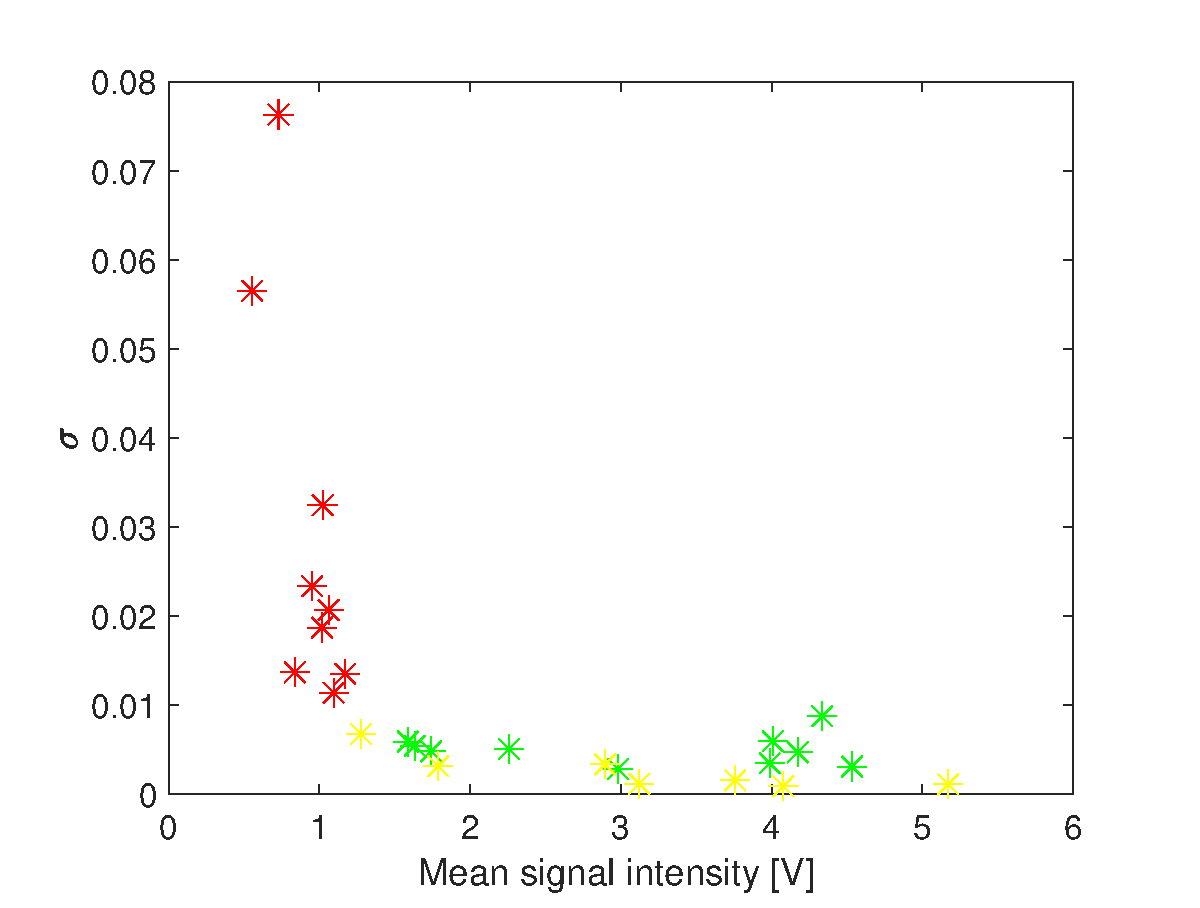
\includegraphics[width=0.7\textwidth]{result/noise/meanV_sigma.eps}
%    \subcaption{}
%    \label{fig:snr_v_sigma}
%\end{minipage}
%\begin{minipage}[t]{0.495\textwidth}
%    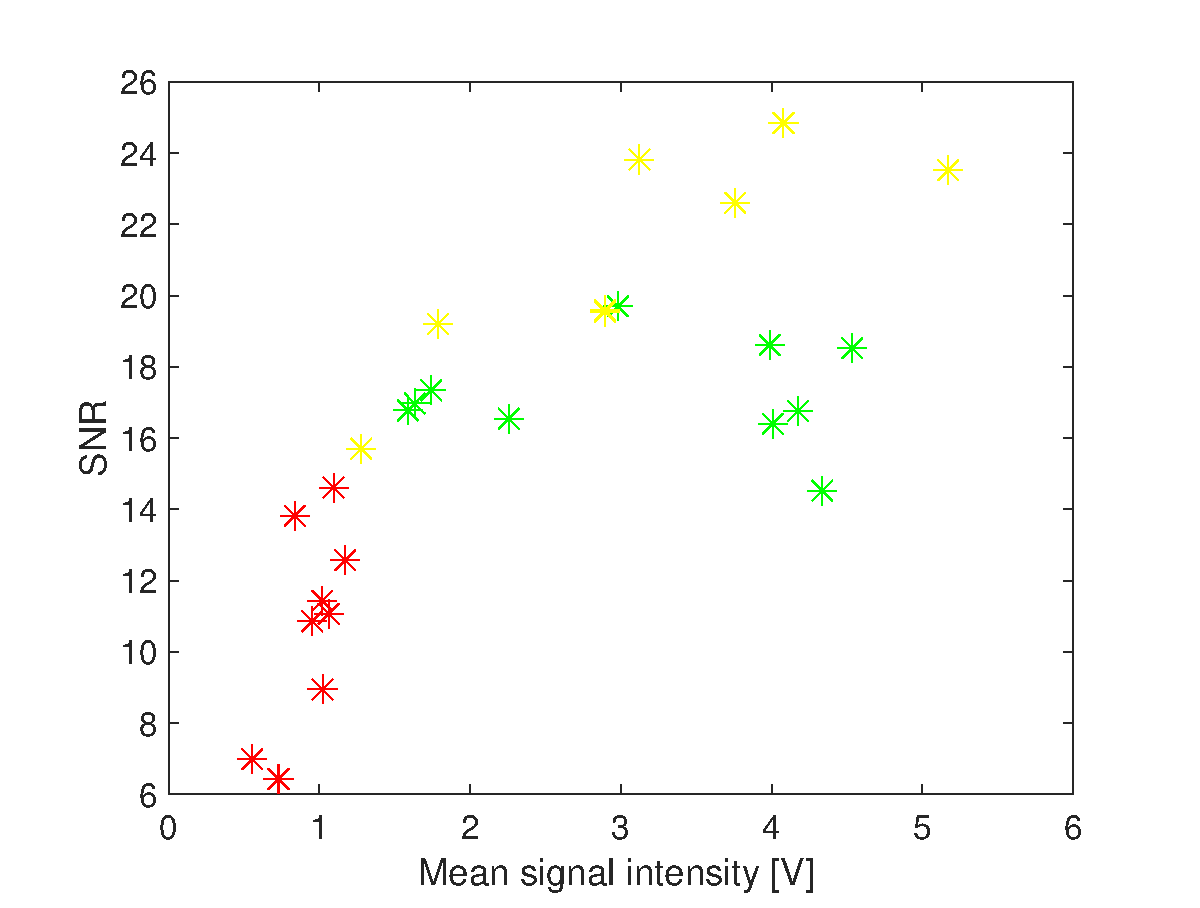
\includegraphics[width = \textwidth]{result/noise/meanV_snr.eps}
%    \subcaption{}
%    \label{fig:snr_v_SNR}
%\end{minipage}
    \caption{Mean sampled signal intensity compared to the normalized background noise variance, each signal has the same corresponding color classification as given before, shown in figure~\ref{fig:brisque_plot}.}
    \label{fig:snr_v_sigma}
\end{figure}

From the plot in figure~\ref{fig:snr_v_sigma}, it can be seen that over approximately 1.2 volt mean signal intensity there are no images from the red image set while images from both the yellow and green image set is mixed over 1.2 volt. Under 1.2 volt mean signal intensity the noise variance to desired signal rapidly increases.


\subsubsection{Luminance Change in scene}
As predicted in section~\ref{sec:Dynamics_in_scene}, dynamics in the scene could result in poor reconstruction performance and an algorithm to suppress the distortion caused by luminance change was tested in the simulated case in section~\ref{sec:dyn_sim}. With an exposure time of just under one minute for the SPC this problem turned out to be constantly present when taking photos of natural scenes outdoors and the luminace change in the signal was more complex then the simulated test case, the sensor was highly sensitive to luminace change. This observation should not be unanticipated, the sensor sums up half the scenes light which make the tiniest intensity change for each pixel a large global change.\\[0.1in] 

In this section the impact of luminnace change on the signal and the results of using the moving mean algorithm (defined in section~\ref{sec:Dynamics_in_scene}) is presented. In figure~\ref{fig:lc_plot} the sampled signal effected by luminance change and the signal proceeded by the moving mean algorithm in blue is shown. 



\begin{figure}[H]
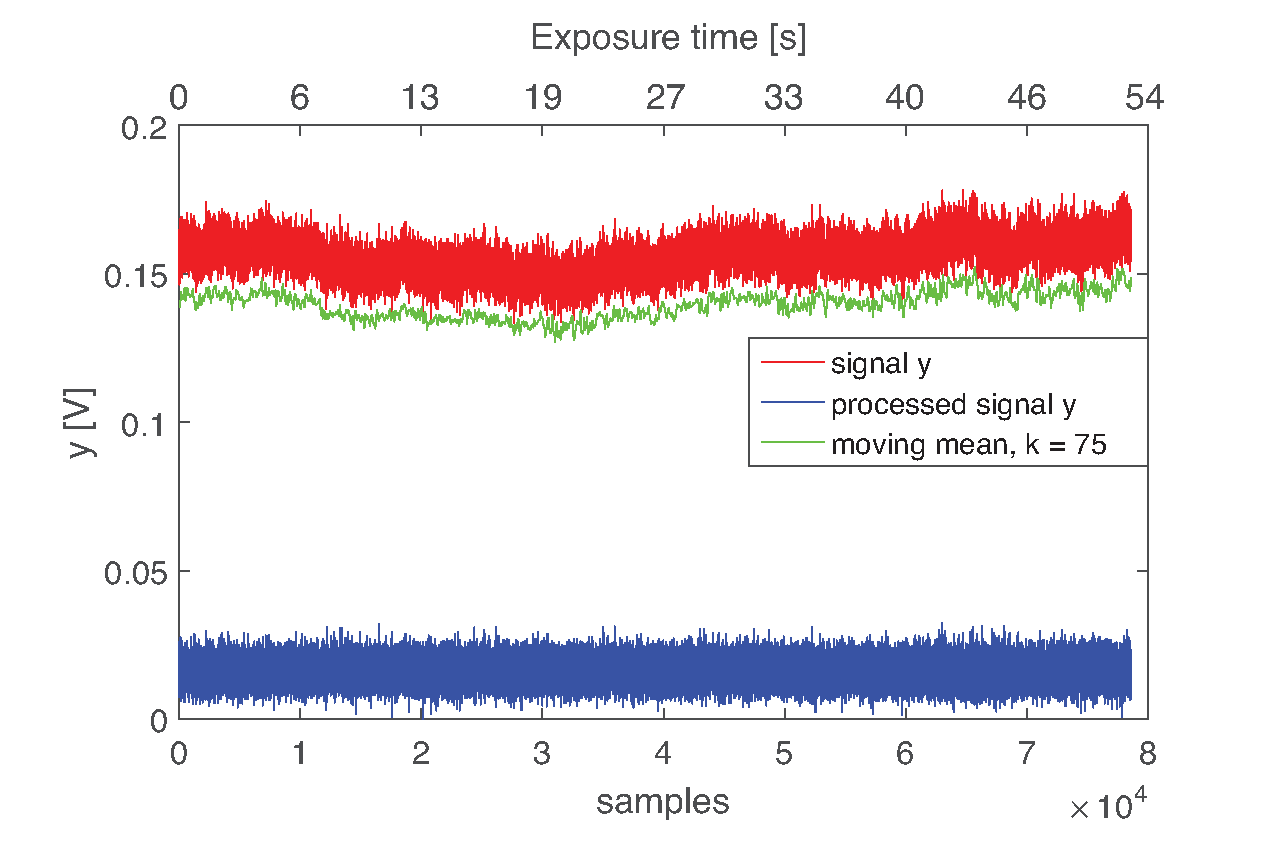
\includegraphics[width = 0.8\linewidth]{result/luminance/li.eps}
	\caption{Sampled signal from SPC with light intensity change and the improved moving mean processed signal.}
	\label{fig:lc_plot}
\end{figure}

As can be seen on the moving mean plotted, the intensity change is very fast and can change in matter of a split of a second, "k" which is the number of neighboring samples to calculate the average  was set to 75 to match the fast change which corresponds to a window of 50 milliseconds.\\[0.1in]

In figure~\ref{fig:lc_image} a reconstructed image without the method used and one with the method used is displayed.

\begin{figure}[H]
\begin{minipage}[t]{0.49\textwidth}

\includegraphics[width = 1\linewidth]{result/luminance/24_512_m30.PNG}
	\subcaption{}
	\label{lc_bf}
\end{minipage}
\begin{minipage}[t]{0.49\textwidth}

\includegraphics[width = 1\linewidth]{gfx/car/car_m30.png}
	\subcaption{}
	\label{lc_af}
\end{minipage}
	\caption{Reconstructed images, (a) before and (b) after applying moving mean average method.}
	\label{fig:lc_image}
\end{figure}

As can be seen in the figure, the method produces good result, the image reconstructed without the signal processing has a severe global noise due to the non stationary signal and the reconstruction performance significantly significantly lower. This images is actually one of the images captured in good conditions with strong lighting and mild intensity change overall.


\subsubsection{Edge response}
The edge response is used to comparing the sharpness of cameras and lenses. The edge response from the SPC is compared to a state of the art SWIR camera. Two scenes was captured by the SPC and a conventional SWIR camera containing printed sheath of paper with simple tilted shapes on them, see figure~\ref{fig:mtf_target}. The scene was lit by a 135 Watt halogen lamp placed two meters from the sheath.



\begin{figure}[H]
    \centering
    
\includegraphics[width=0.8\linewidth]{result/mtf/Target.eps}
    \caption{Printed targets with markings where the edge response measurements was performed}
    \label{fig:mtf_target}
\end{figure}

In the resulting images, edge response measurements was gathered from the specified edges in figure~\ref{fig:mtf_target}, with the result from all edges and both images for respective cameras, a mean and standard deviation is calculated. For the SPC, images reconstructed from 5\% to 30\% was tested in order to see if the subsampling ratio effected the MTF result. In figure~\ref{fig:mtf_target_im} the images from the SWIR camera and SPC are presented.

\begin{figure}[H]
    \centering
\begin{minipage}[t]{0.49\textwidth}
    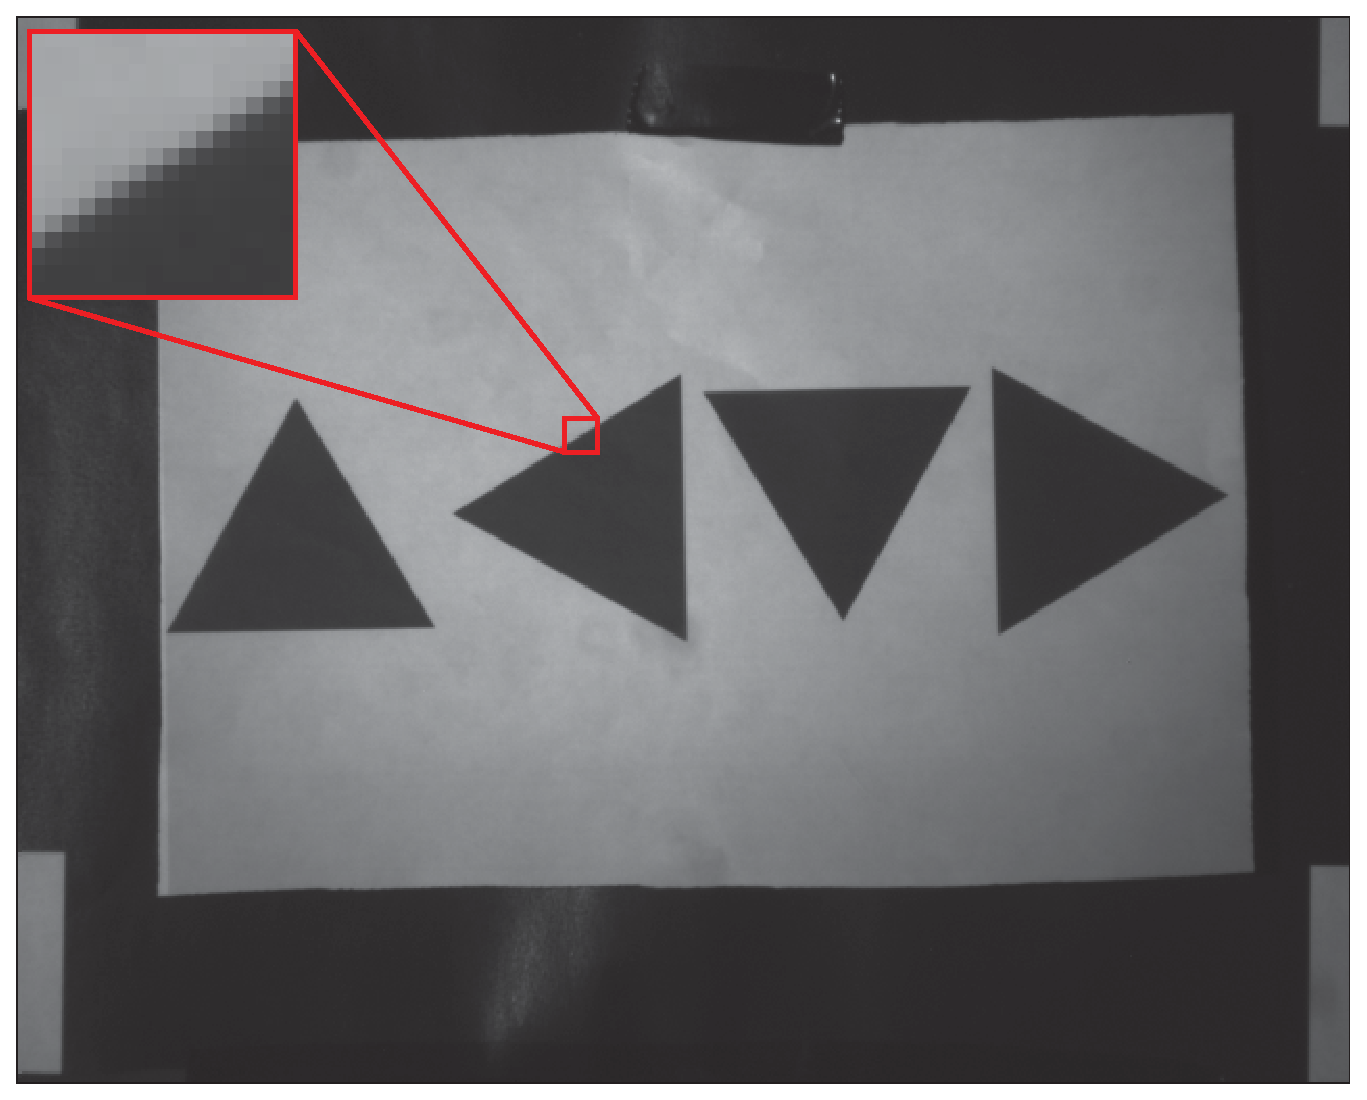
\includegraphics[width=1\textwidth]{result/mtf/swir22.eps}
    \subcaption{}
    \label{fig:mtf_s2}
\end{minipage}
\begin{minipage}[t]{0.49\textwidth}
    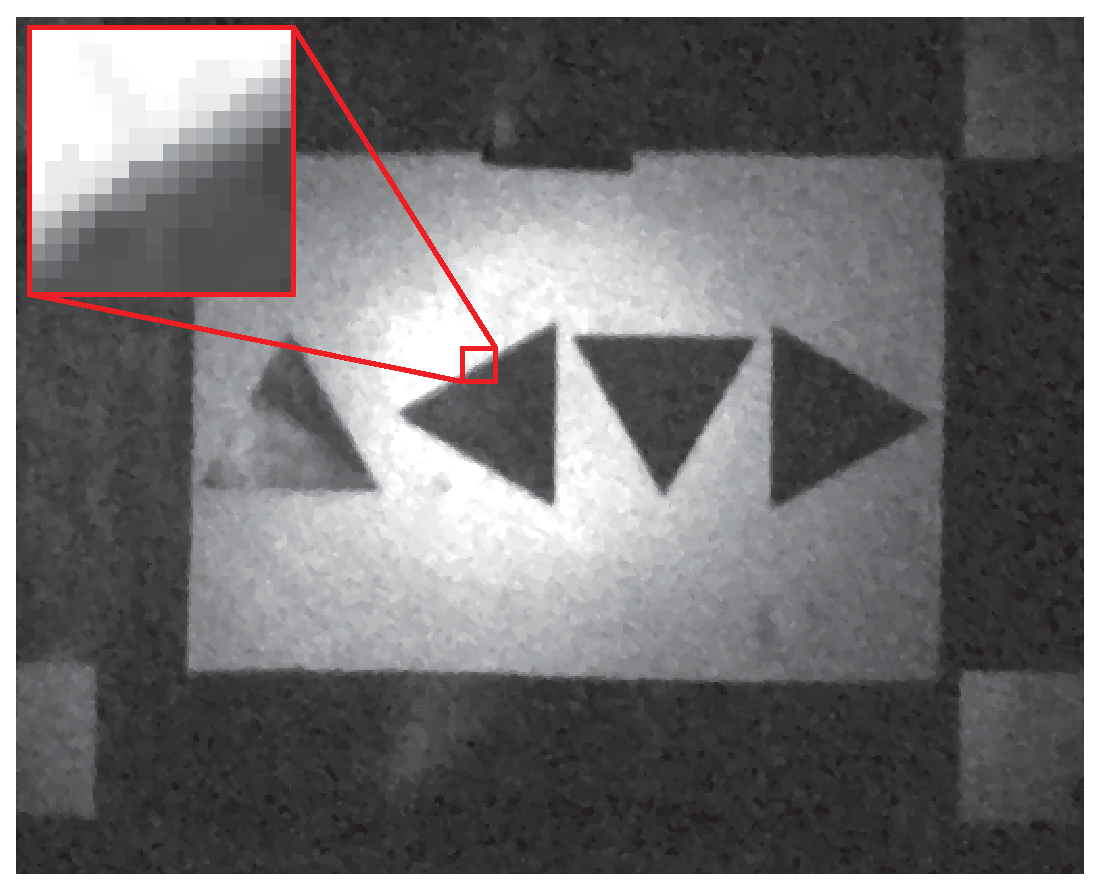
\includegraphics[width=1\textwidth]{result/mtf/spc222.eps}
    \subcaption{}
    \label{fig:mtf_spc2}
\end{minipage}
\begin{minipage}[t]{0.49\textwidth}
    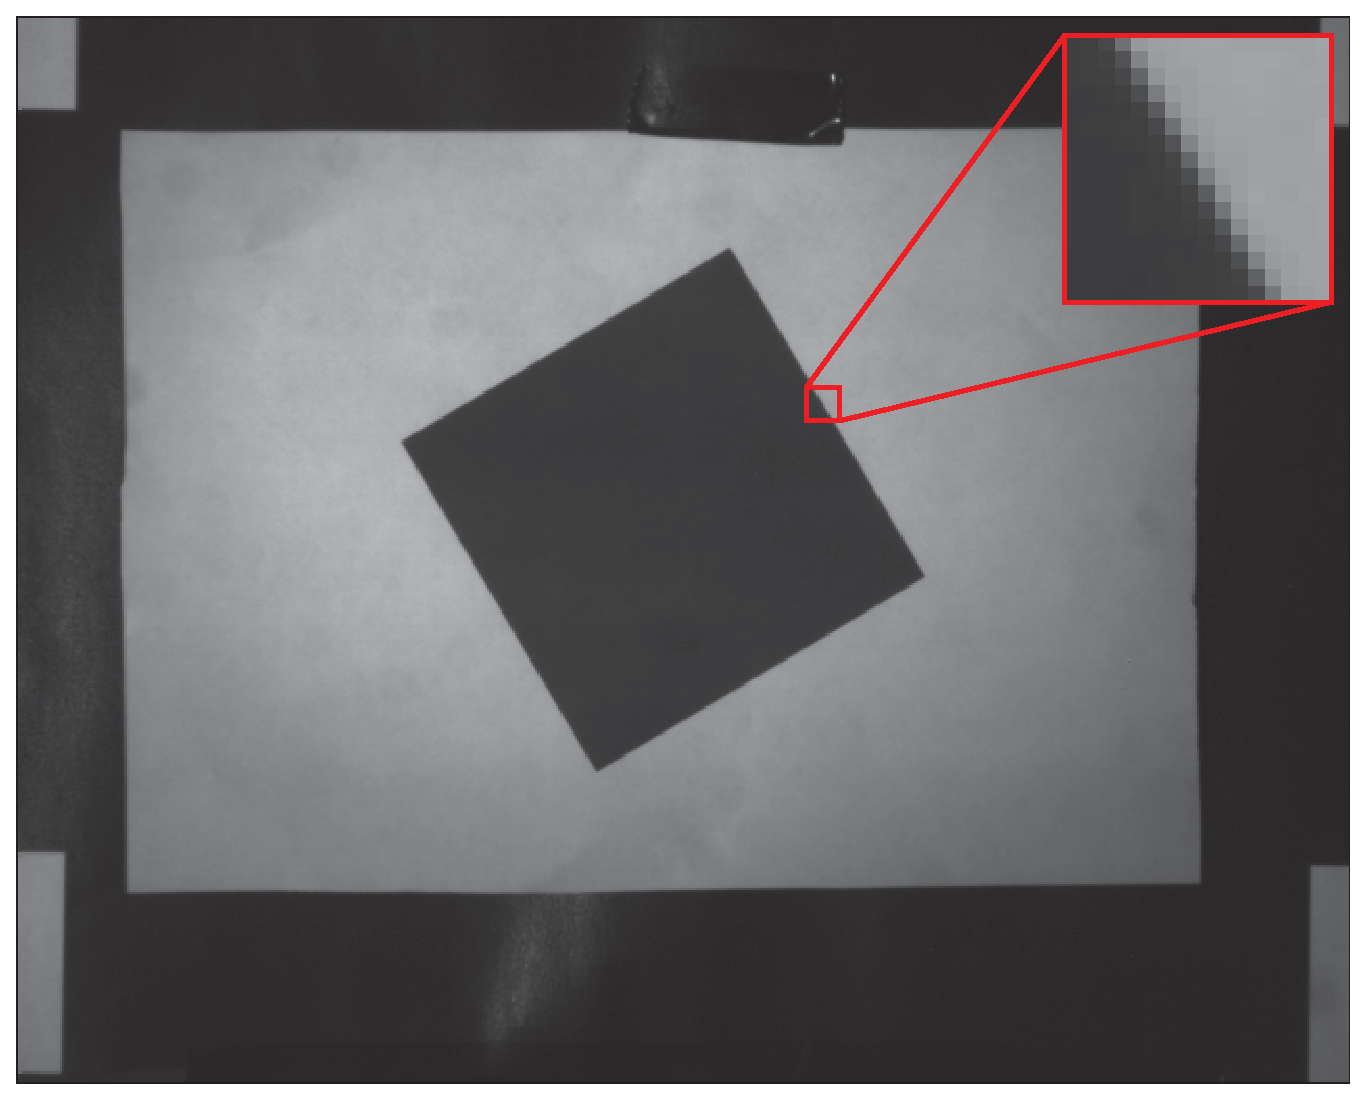
\includegraphics[width=1\textwidth]{result/mtf/swir12.eps}
    \subcaption{}
    \label{fig:mtf_s1}
\end{minipage}
\begin{minipage}[t]{0.49\textwidth}
    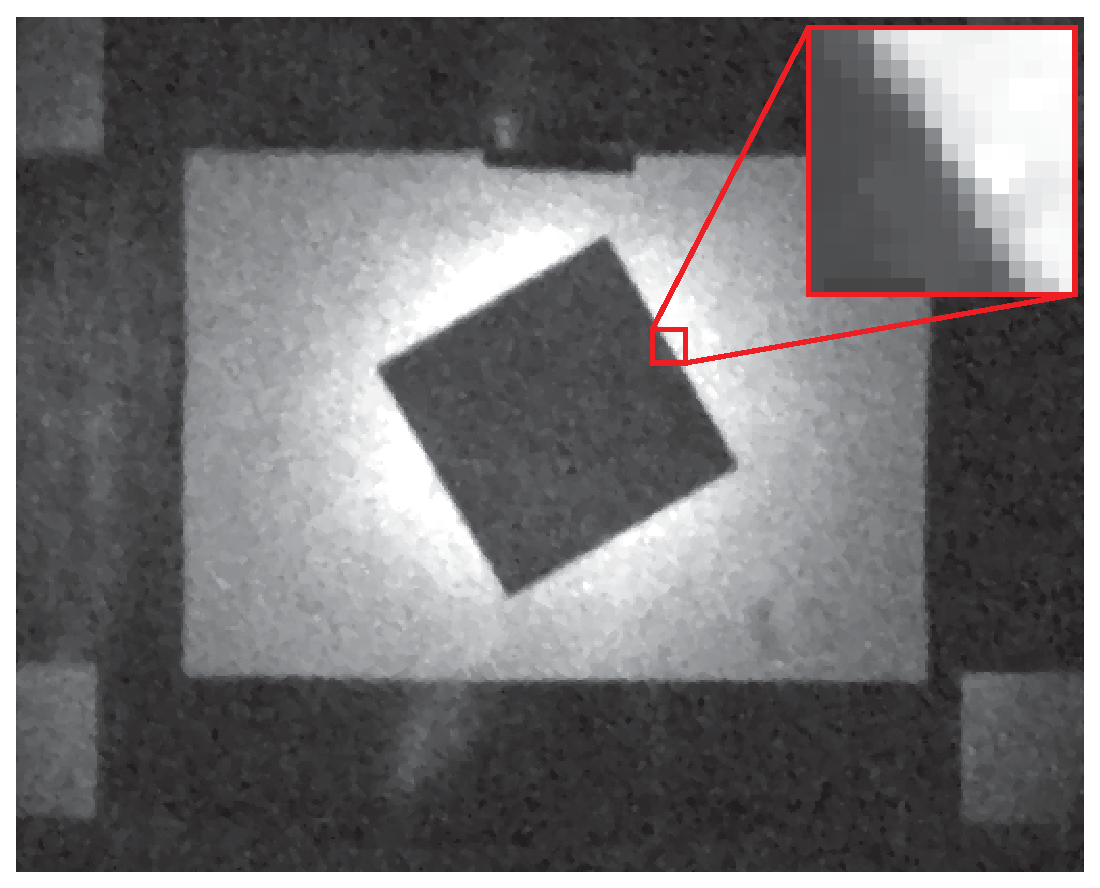
\includegraphics[width=1\textwidth]{result/mtf/spc122.eps}
    \subcaption{}
    \label{fig:mtf_spc1}
\end{minipage}
    \caption{SPC and state of the art SWIR camera images. (a) and (c) from the conventional SWIR camera and (b) and (c) captured with the SPC.}
    \label{fig:mtf_target_im}
\end{figure}




The edge response is measured in the distance (pixels) required for a edge to rise from $10\%$ to $90\%$ intensity change. In figure~\ref{fig:rise} the result from the experiment in presented. 

\begin{figure}[H]
    \centering
    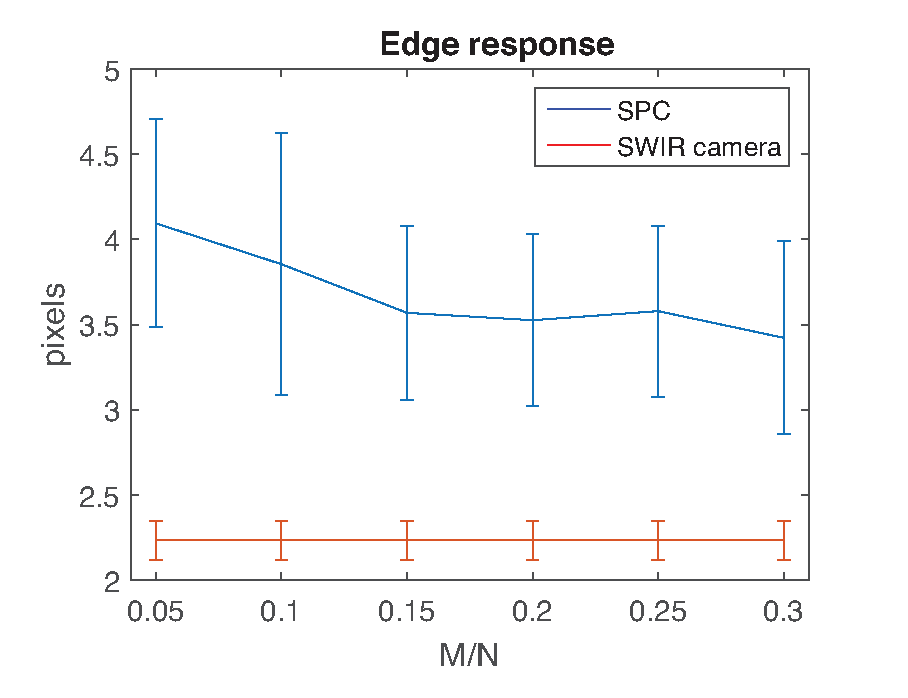
\includegraphics[width=0.7\linewidth]{result/mtf/Rise10_90.eps}
    \caption{Edge response, distance (pixels) to rise from 10-90\% in average for an edge.}
    \label{fig:rise}
\end{figure}

From the plot in figure~\ref{fig:rise}, a clear difference between the SPC and state of the art SWIR camera can be seen, where the conventional SWIR camera has in average half the distance against the SPC images. Some improvement is seen when the subsample ratio is increased, but the standard deviation is almost constant, meaning that the difference between the state of the art SWIR camera and the SPC, in best case only differ about 0.5 pixels, but in the worst case differ about 1.7 pixels and in average 1.2 pixel.

\subsubsection{Subsampling ratio}
\label{sec:measurements}
From the theory of compressive sensing the number of measurements needed to reconstruct an image is correlated with the sparsity or compressibility of the image, therefore it is hard to give a good estimate of a subsampling ratio needed to obtain a desired quality of the reconstruction. In addition, using a SPC where noise contaminate the signal and the scene may not be completely stationary, the number of measurements needed will increase in proportion to the noise and the change in the scene. In this subsection the minimum subsampling ratio will be presented followed by how the reconstructed image quality is effected by an increese of subsampling ratio.\\[0.1in]


The minimum number of measurements to reconstruct a image where the motive can be recognized is also effected by the factors described, trying to reconstruct an image under the minimum subsampling ratio results in an image with just noise. A survey of the minimum subsampling ratio was performed on all images captured by the SPC in this thesis, and the result ranged from 2\% to 4\% to obtain a recognizable images, in figure~\ref{fig:minimum_fig} a sample of three images with varying minimum subsambling ratios is displayed.


\begin{figure}[H]
\begin{minipage}[t]{0.32\linewidth} %Car
	
\includegraphics[width = 1\linewidth]{result/minimum/24_512_m2.PNG}
	\subcaption{Subsampling ratio 2\%.}
	\label{fig:minimum_car}
\end{minipage}
\begin{minipage}[t]{0.32\linewidth} % Hus
	
\includegraphics[width = 1\linewidth]{result/minimum/37_512_m3.PNG}
	\subcaption{Subsampling ratio 3\%.}
	\label{fig:minimum_house}
\end{minipage}
\begin{minipage}[t]{0.32\linewidth} %Sit
	
\includegraphics[width = 1\linewidth]{result/minimum/64_512_m3.PNG}
	\subcaption{Subsampling ratio 3\%.}
	\label{fig:minimum_forest}
\end{minipage}
	\caption{Varying minimum subsampling ratios to reconstruct sample images captured by the SPC.}
	\label{fig:minimum_fig}
\end{figure}

In the sample images in figure~\ref{fig:minimum_fig} the minimum subsampling ratio varied between 2\% to 3\%, but as can be seen, this is only the minimum subsampling ratio where the motive is merely recognizable, large structure can be identified but detail is lost. In general a subsampling ratio of 5\% has always succeeded to reconstruct a identifiable image with some fine details, moving along this topic the results from higher subsampling ratios is presented.\\[0.1in]

In figure~\ref{fig:subsampling_ratios} three scenes is reconstructed using different subsample ratios ranging from 5\% to 30\%, for each row the subsampling ratio is increased by 5\% and at the top a reference image from a visual camera is presented. What should be expected is increased image quality with increased subsampling ratio, this result can give an perception of which subsampling ratio is good enough for a given purpose, and as can be seen, the increase of subsampling ratio is not linear proportional to the increase in perceived image quality, just like regular image compression.
     

\begin{figure}[H]
\begin{minipage}[t]{0.3\linewidth} %Car
	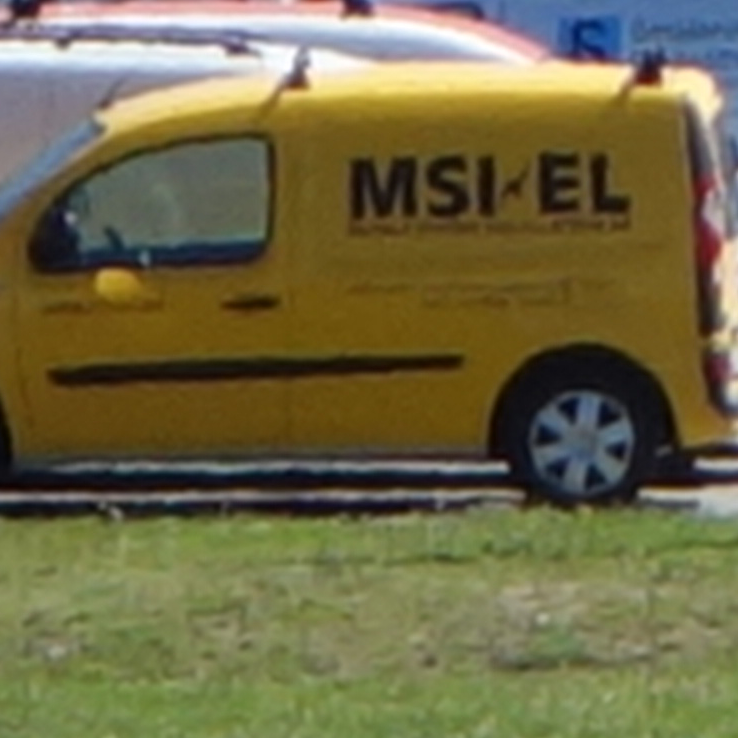
\includegraphics[width = 1\linewidth]{gfx/car/car_org.png}
	%\subcaption{Visual camera image.}
	\label{fig:car_org}
\end{minipage}
\begin{minipage}[t]{0.3\linewidth} % Hus
	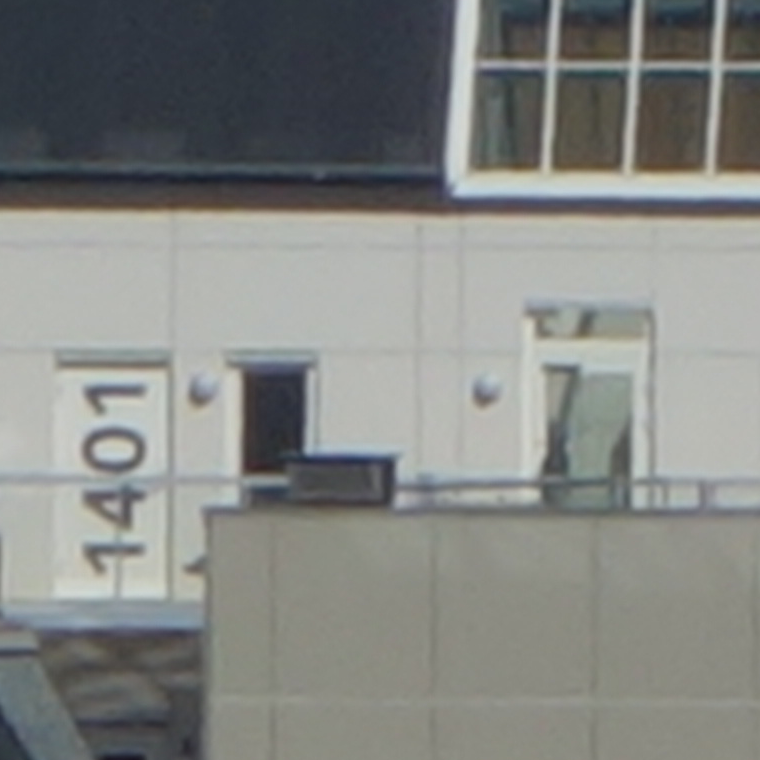
\includegraphics[width = 1\linewidth]{gfx/hus/hus_org.png}
	\subcaption{Visual camera image.}
	\label{fig:hus_org}
\end{minipage}
\begin{minipage}[t]{0.3\linewidth} %Sit
	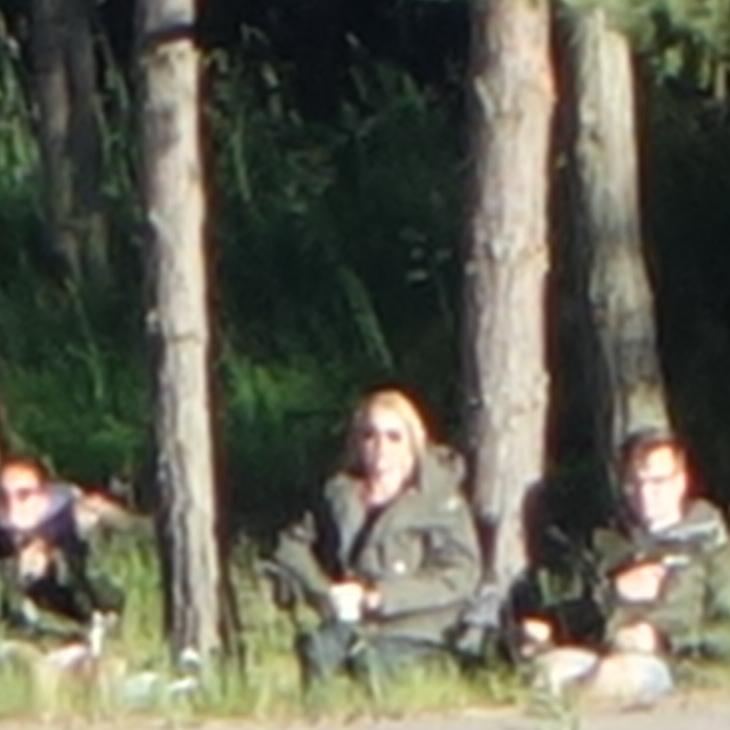
\includegraphics[width = 1\linewidth]{gfx/sit/sit_org.png}
	%\subcaption{}
	\label{fig:sit_org}
\end{minipage}
\begin{minipage}[t]{0.3\linewidth} %Car
	
\includegraphics[width = 1\linewidth]{gfx/car/car_m5.png}
	%\subcaption{Subsampling ratio 5\%}
	\label{fig:car_m5}
\end{minipage}
\begin{minipage}[t]{0.3\linewidth} % Hus
	
\includegraphics[width = 1\linewidth]{gfx/hus/hus_m5.png}
	\subcaption{Subsampling ratio 5\%}
	\label{fig:hus_m5}
\end{minipage}
\begin{minipage}[t]{0.3\linewidth} %Sit
	
\includegraphics[width = 1\linewidth]{gfx/sit/sit_m5.png}
	%\subcaption{}
	\label{fig:sit_m5}
\end{minipage}
\begin{minipage}[t]{0.3\linewidth} %Car
	
\includegraphics[width = 1\linewidth]{gfx/car/car_m10.png}
	%\subcaption{Subsampling ratio 10\%}
	\label{fig:car_m10}
\end{minipage}
\begin{minipage}[t]{0.3\linewidth} % Hus
	
\includegraphics[width = 1\linewidth]{gfx/hus/hus_m10.png}
	\subcaption{Subsampling ratio 10\%}
	\label{fig:hus_m10}
\end{minipage}
\begin{minipage}[t]{0.3\linewidth} %Sit
	
\includegraphics[width = 1\linewidth]{gfx/sit/sit_m10.png}
	%\subcaption{}
	\label{fig:sit_m10}
\end{minipage}
\begin{minipage}[t]{0.3\linewidth} %Car
	
\includegraphics[width = 1\linewidth]{gfx/car/car_m15.png}
	%\subcaption{Subsampling ratio 15\%}
	\label{fig:car_m15}
\end{minipage}
\begin{minipage}[t]{0.3\linewidth} % Hus
	
\includegraphics[width = 1\linewidth]{gfx/hus/hus_m15.png}
	\subcaption{Subsampling ratio 15\%}
	\label{fig:hus_m15}
\end{minipage}
\begin{minipage}[t]{0.3\linewidth} %Sit
	
\includegraphics[width = 1\linewidth]{gfx/sit/sit_m15.png}
	%\subcaption{}
	\label{fig:sit_m15}
\end{minipage}
\end{figure}
\begin{figure}[H]
\ContinuedFloat
\begin{minipage}[t]{0.3\linewidth} %Car
	
\includegraphics[width = 1\linewidth]{gfx/car/car_m20.png}
	%\subcaption{Subsampling ratio 20\%}
	\label{fig:car_m20}
\end{minipage}
\begin{minipage}[t]{0.3\linewidth} % Hus
	
\includegraphics[width = 1\linewidth]{gfx/hus/hus_m20.png}
	\subcaption{Subsampling ratio 20\%}
	\label{fig:hus_m20}
\end{minipage}
\begin{minipage}[t]{0.3\linewidth} %Sit
	\includegraphics[width = 1\linewidth]{gfx/sit/sit_m20.png}
	%\subcaption{}
	\label{fig:sit_m20}
\end{minipage}
\begin{minipage}[t]{0.3\linewidth} %Car
	\includegraphics[width = 1\linewidth]{gfx/car/car_m25.png}
	%
	\label{fig:car_m25}
\end{minipage}
\begin{minipage}[t]{0.3\linewidth} % Hus
	\includegraphics[width = 1\linewidth]{gfx/hus/hus_m25.png}
	\subcaption{Subsampling ratio 25\%}
	\label{fig:hus_m25}
\end{minipage}
\begin{minipage}[t]{0.3\linewidth} %Sit
	\includegraphics[width = 1\linewidth]{gfx/sit/sit_m25.png}
	%\subcaption{}
	\label{fig:sit_m25}
\end{minipage}
\begin{minipage}[t]{0.3\linewidth} %Car
	\includegraphics[width = 1\linewidth]{gfx/car/car_m30.png}
	%\subcaption{Subsampling ratio 30\%}
	\label{fig:car_m30}
\end{minipage}
\begin{minipage}[t]{0.3\linewidth} % Hus
	\includegraphics[width = 1\linewidth]{gfx/hus/hus_m30.png}
	\subcaption{Subsampling ratio 30\%}
	\label{fig:hus_m30}
\end{minipage}
\begin{minipage}[t]{0.3\linewidth} %Sit
	\includegraphics[width = 1\linewidth]{gfx/sit/sit_m30.png}
	%\subcaption{}
	\label{fig:sit_m30}
\end{minipage}
	\caption{Reconstructed images captured by the SPC with increasing subsampling ratios. First row showing a reference visual spectrum image followed by SPC images reconstructed with 5\% from top then increased subsampling ratio by 5\% for each row to 30\% on the last row.}
	\label{fig:subsampling_ratios}
\end{figure}

The are a few thinks that can be noted in the images in figure~\ref{fig:subsampling_ratios}, 

\begin{itemize}
\item the reconstructed images behave as expected, when the subsample ratio increases the image quality increases. 

\item Already at 5\% subsampling ratio the scene can be properly identified unlike the case in minimal subsamples ratio. The images has some artifacts that can be linked to the reconstruction algorithm, the images looks like the made of small patches.

\item Between 10-15\% the finer details start to appear, like the gap between the panels in the facade, the text on the car and door are getting sharper and the structure of the faces start to appear.

\item As stated before, the image quality does not increase at the same rate as the subsampling ratio, this is most noticeable when increasing the subsampling ratio above 15\%. The improvement after 15\% is not as easy to spot as from the increments before, but they can be found in the details. 
\end{itemize}



 





